\section{Experiment} \label{sec:experiment}
This section describes the experiment conducted to address the Research Questions. As in typical methodologies used in ML studies, it comprises the following steps: Data Collection (\ref{subsec:collection}), Data Preprocessing (Section \ref{subsec:preprocessing}), and Training and Testing (Section \ref{subsec:training}).

\subsection{Data Collection} 	\label{subsec:collection}
This step in the experimental research encompasses selecting FLOSS datasets to serve as the data source, studying and interpreting its data structure, and finally extracting relevant data from its repository (feature extraction). In this research, Cassandra, Hadoop, Linux, Mozilla, and Spark Open Systems were considered as potential Open Source Systems to study. In a first approximation, Cassandra, Hadoop and Spark were selected as data sources of CR records, due to the fact they are open, well stablished, have a considerable number of CRs already registered, use standard repositories, and were under study by other researchers in our research group.

Cassandra[cassandra.apache.org] is a distributed NoSQL database management system designed to handle large amounts of data across many servers, providing fault-tolerance with no single point of failure. Hadoop[hadoop.apache.org] is a framework that allows for the distributed processing of large data sets across clusters of computers using simple programming models. Spark[spark.apache.org] is a cluster-computing engine for large-scale data processing which provides an interface for programming entire clusters with implicit data parallelism and fault-tolerance. They are considered a specialized and complex FLOSS project with many users with different levels of expertise.

CRs from these FLOSS projects are stored in a Jira based repository [\url{https://www.atlassian.com/software/jira}] which allows for access to all CR contents in XML format. Everything is available (except change history), from CR long description field (with lines with few characters to ones with many lines), including code snippets and exception stack trace. Two steps are used to perform data extraction from their web site[\url{http://issues.apache.org}]: (i) copying CR basic data (e.g. status and resolution) from XML contents; and (ii) copying CR changes history from external HTML pages (this may be important for learning).

CR record data from February 01, 2006 to May 07, 2017 were collected.  The total number of CR records retrieved after preprocessing was 22901. 
 
\begin{figure*}[!ht]
  \centering
  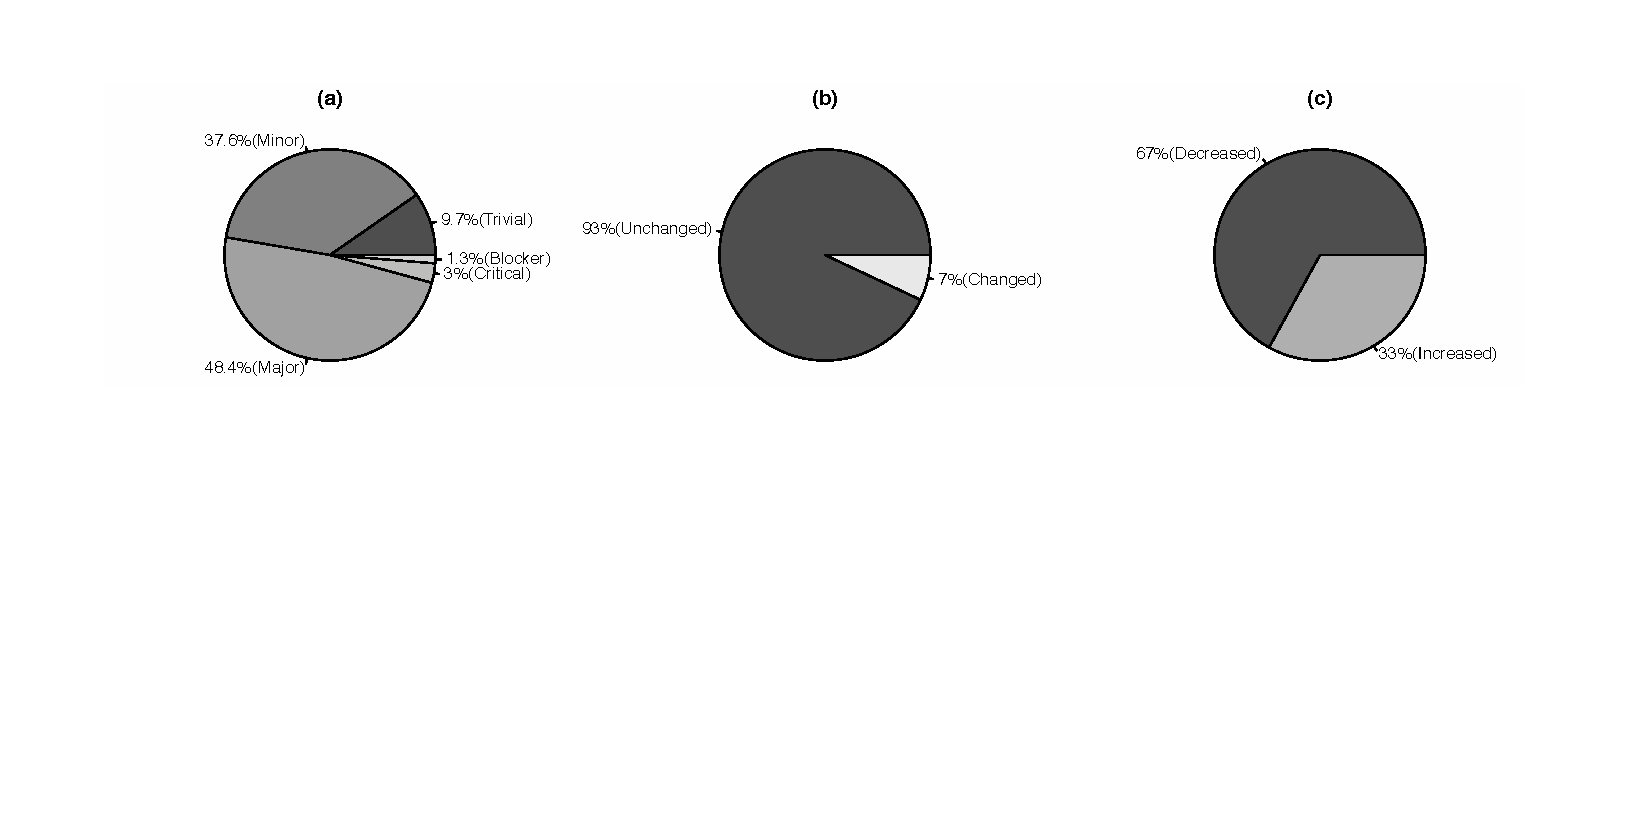
\includegraphics[scale=0.7]{figures/issues_distribution_cassandra.pdf}    
  \caption{Cassandra dataset distributions: (a) severity level (b) change pattern (c) direction of change.}
  \label{fig:issues_distribution_cassandra}
\end{figure*}

\begin{figure*}[!ht]
  \centering
  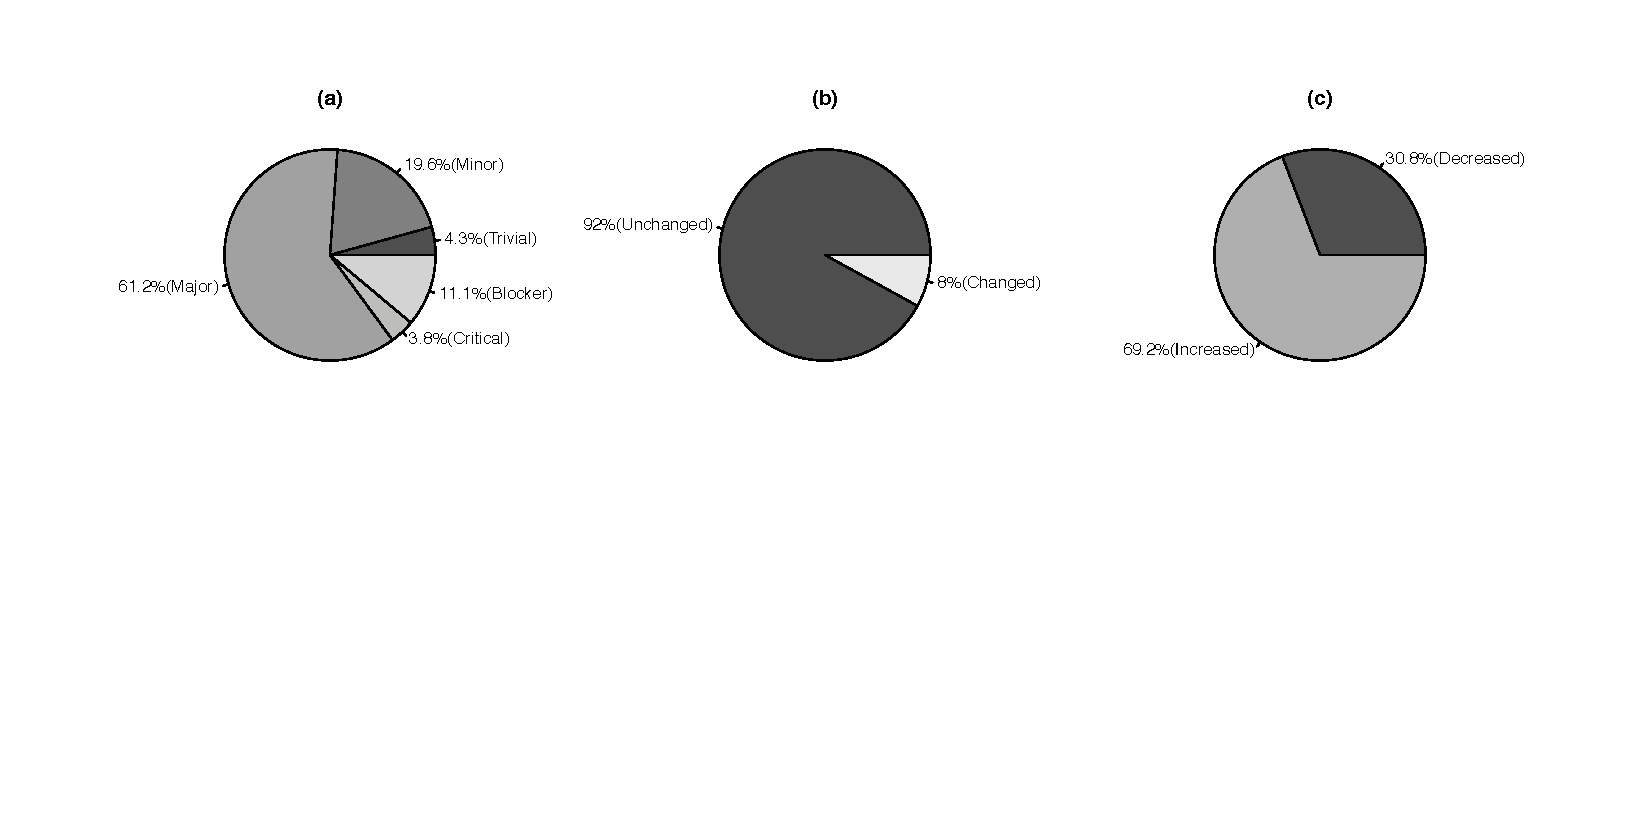
\includegraphics[scale=0.7]{figures/issues_distribution_hadoop.pdf}
  \caption{Hadoop dataset distributions: (a) severity level (b) change pattern (c) direction of change.}
  \label{fig:issues_distribution_hadoop}
\end{figure*}

\begin{figure*}[!ht]
  \centering
  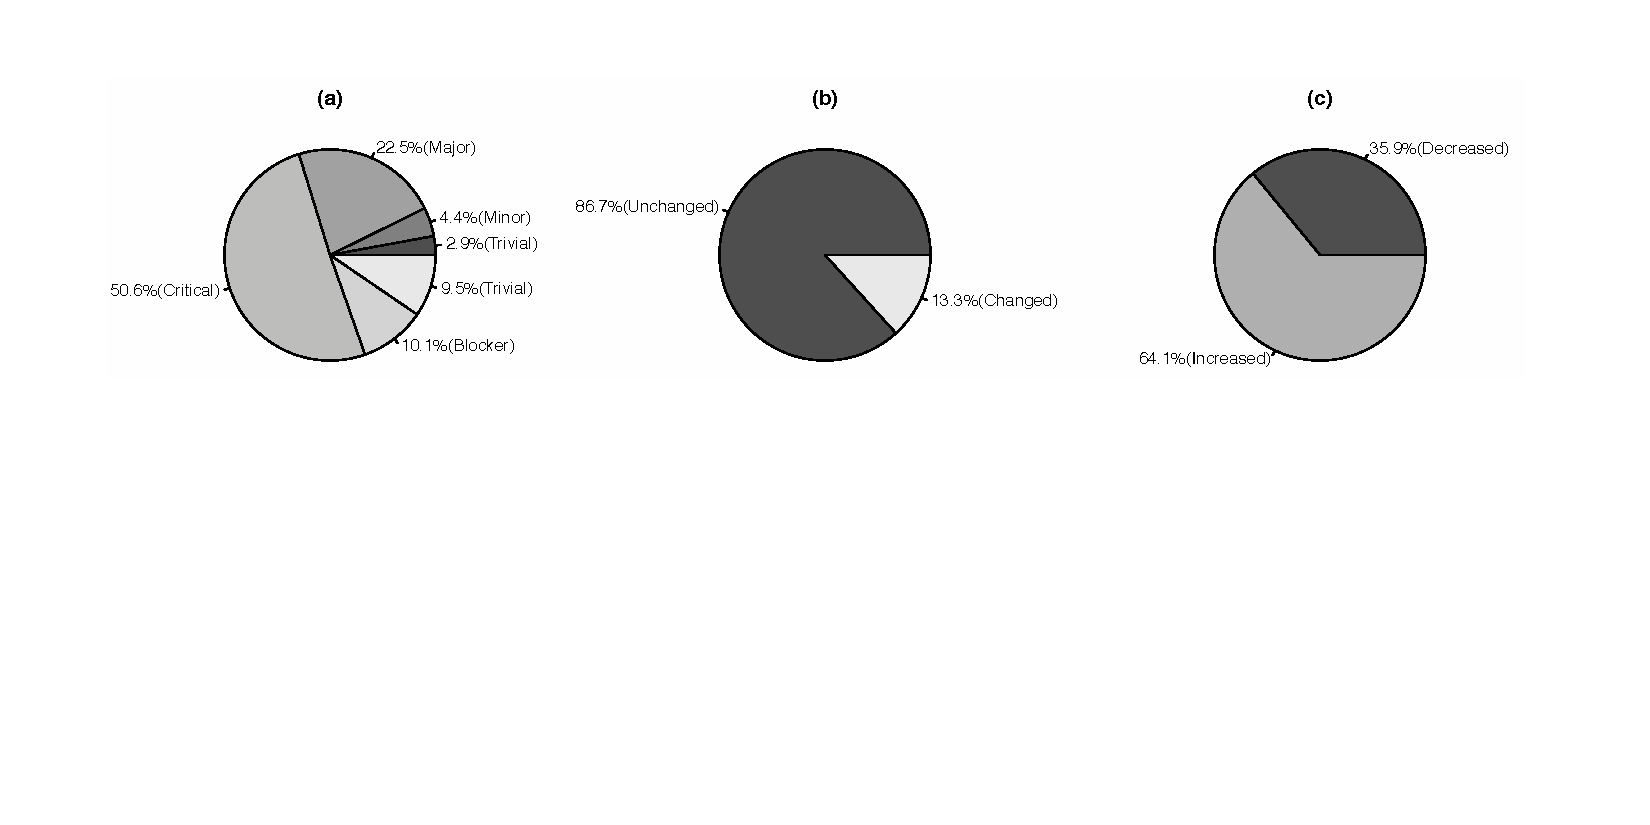
\includegraphics[scale=0.7]{figures/issues_distribution_spark.pdf}   
  \caption{Spark dataset distributions: (a) severity level (b) change pattern (c) direction of change.}
  \label{fig:issues_distribution_spark}
\end{figure*}


Figure \ref{fig:issues_distribution_cassandra} shows how the 7538 retrieved CR Cassandra records were distributed in terms of severity level and severity level change. Figure \ref{fig:issues_distribution_cassandra}(a) shows the severity level distribution: 9.7\% have severity trivial (1); 37.6\% have severity minor (2); 48.4\% have severity major (3), 3.0\% have severity critical (4), and 1.3\% have severity blocker (5). Figure \ref{fig:issues_distribution_cassandra}(b) shows that only 7.0\% have changed their severities levels during the CR lifecycle. Finally, Figure \ref{fig:issues_distribution_cassandra}(c) reveals that of these 7.0\% CRs which changed their severity, 67\% decreased it, and 33\% increased it. 

Figure \ref{fig:issues_distribution_hadoop} shows how the 8262 retrieved CR Hadoop records from were distributed in terms of severity level and severity level change. Figure \ref{fig:issues_distribution_hadoop}(a) shows the severity level distribution: 4.3\% have severity trivial (1); 19.6\% have severity minor (2); 61.2\% have severity major (3), 3.8\% have severity critical (4), and 11.1\% have severity blocker (5). Figure \ref{fig:issues_distribution_hadoop}(b) shows that only 8.0\% have changed their severities levels during the CR lifecycle. Finally, Figure \ref{fig:issues_distribution_hadoop}(c) reveals that of these 8.0\% CRs which changed their severity, 30.8\% decreased it, and 69.2\% increased it. 

Figure \ref{fig:issues_distribution_spark} shows how the 7101 retrieved CR Spark records were distributed in terms of severity level and severity level change. Figure \ref{fig:issues_distribution_spark}(a) shows the severity level distribution: 2.9\% have severity trivial (1); 4.4\% have severity minor (2); 22.5\% have severity major (3), 50.6\% have severity critical (4), and 10.1\% have severity blocker (5). Figure \ref{fig:issues_distribution_spark}(b) shows that only 13.3\% have changed their severities levels during the CR lifecycle. Finally, Figure \ref{fig:issues_distribution_spark}(c) reveals that of these 13.3\% CRs which changed their severity, 35.9\% decreased it, and 64.1\% increased it. 

Summarizing findings in Figures \ref{fig:issues_distribution_cassandra}, \ref{fig:issues_distribution_hadoop} and  \ref{fig:issues_distribution_spark}: (a) the most frequent severity level type is ``major''; (b) there have been few changes in severity levels; (c) in two of them (Hadoop and Spark), severity levels increased. Furthermore, one can see that these datasets are clearly imbalanced, posing additional difficulty to the application of the ML methodology. 

\subsection{Preprocessing} 	\label{subsec:preprocessing}

Raw data previously collected from the Cassandra, Hadoop and Spark CR repositories were not properly structured to serve as input to ML algorithms, they weren't in tidy data format \cite{DeJonge2013}. The classical way to address this problem is to run preprocessing procedures to extract, organize and structure relevant features out of the raw data. Specific scripts were written in R language to accomplish this features extraction. Preprocessing tasks were executed as follows:  

\begin{itemize}
 \item Extraction of relevant features: key, type, status, resolution status, days to resolve, quantity of comments, severity level and long description of CRs; 
 \item Selecting only CRs with status equals to Closed and resolution equals to Fixed and Implemented. This type of CRs was effectively implemented by the development team and they can no longer have their severity level changed.
 \item Merging CR features with their change history data. This additional information allows for the identification of CRs that have changed severity level during the CR lifecycle, and furthermore, if they have changed for better (decrease) or worse (increase).
 \item Performing text mining in the long description field to identify the 100 most frequent words. This information is then converted into features for each CR.
\end{itemize}

\subsection{Training and testing}  	\label{subsec:training}

Training and testing steps start with partitioning the already preprocessed dataset in two disjoint subsets: a subset for training, with 80\% of the CRs, and a subset for testing, with the remaining 20\% of the CRs. Three classical sampling approaches, random, proportional, and uniform\cite{Japkowicz:2011} were analyzed to select the training set. Best results were obtained with the random sampling technique. In the training phase, we have used the 5$\times$3 Repeated Cross-Validation technique \cite{Zhao2013} to obtain more stable estimates of each algorithm's performance and enhance replicability of the results \cite{Japkowicz:2011}. In the testing phase, each ML algorithm was validated with 20\% of each CR dataset to measure its accuracy.
 
We have chosen three traditional ML algorithms: Neural Networks\cite{Haykin:1998}, Random Forest\cite{Breiman2001} and Support Vector Machine(SVM)\cite{Cristianini:1999} which were implemented, respectively, using neuralnet (with Single Hidden Layer), randomForest, and kernlab (with Radial Basis Function Kernel and multi-class classification) R libraries.



